%8 pages
%%
%% This is file `sample-sigconf.tex',
%% generated with the docstrip utility.
%%
%% The original source files were:
%%
%% samples.dtx  (with options: `sigconf')
%% 
%% IMPORTANT NOTICE:
%% 
%% For the copyright see the source file.
%% 
%% Any modified versions of this file must be renamed
%% with new filenames distinct from sample-sigconf.tex.
%% 
%% For distribution of the original source see the terms
%% for copying and modification in the file samples.dtx.
%% 
%% This generated file may be distributed as long as the
%% original source files, as listed above, are part of the
%% same distribution. (The sources need not necessarily be
%% in the same archive or directory.)
%%
%% The first command in your LaTeX source must be the \documentclass command.
%\documentclass[sigconf,table,anonymous]{acmart}
\documentclass[10pt,sigconf]{acmart}

\usepackage{algpseudocode}
\usepackage{algorithm}
\usepackage{algorithmicx}
\usepackage{verbatim}
\usepackage{mathtools}
\usepackage{multirow}
\usepackage{subcaption}
\usepackage{colortbl}
\usepackage{balance}

\usepackage{dirtree}

\usepackage{tikz}
\usetikzlibrary{automata,positioning}
\usetikzlibrary{decorations.pathmorphing}
\tikzset{snake it/.style={decorate, decoration=snake}}

\definecolor{lightgray}{gray}{0.9}


%\def\BibTeX{{\rm B\kern-.05em{\sc i\kern-.025em b}\kern-.08em
	%	T\kern-.1667em\lower.7ex\hbox{E}\kern-.125emX}}

\usepackage{booktabs} % For formal tables

\usepackage{kbordermatrix} % include package @ document preamble
\renewcommand{\kbldelim}{(} % change default array delimiters to parentheses
\renewcommand{\kbrdelim}{)}

\newlength\Origarrayrulewidth

% horizontal rule equivalent to \cline but with 2pt width
\newcommand{\Cline}[1]{%
	\noalign{\global\setlength\Origarrayrulewidth{\arrayrulewidth}}%
	\noalign{\global\setlength\arrayrulewidth{3pt}}\cline{#1}%
	\noalign{\global\setlength\arrayrulewidth{\Origarrayrulewidth}}%
}

% draw a vertical rule of width 2pt on both sides of a cell
\newcommand\Thickvrule[1]{%
	\multicolumn{1}{!{\vrule width 2pt}c!{\vrule width 2pt}}{#1}%
}

% draw a vertical rule of width 2pt on the left side of a cell
\newcommand\Thickvrulel[1]{%
	\multicolumn{1}{!{\vrule width 2pt}c}{#1}%
}

% draw a vertical rule of width 2pt on the right side of a cell
\newcommand\Thickvruler[1]{%
	\multicolumn{1}{c!{\vrule width 2pt}}{#1}%
}

\newcommand\mc{\multicolumn{1}{c}{\cellcolor{lightgray}\textbf{1}}}

%%
%% \BibTeX command to typeset BibTeX logo in the docs
\AtBeginDocument{%
	\providecommand\BibTeX{{%
			\normalfont B\kern-0.5em{\scshape i\kern-0.25em b}\kern-0.8em\TeX}}}

%% Rights management information.  This information is sent to you
%% when you complete the rights form.  These commands have SAMPLE
%% values in them; it is your responsibility as an author to replace
%% the commands and values with those provided to you when you
%% complete the rights form.
\setcopyright{acmcopyright}
\copyrightyear{2021}
\acmYear{2021}
\acmConference[SIGMOD'21]{}{}{}
\acmBooktitle{}
\acmPrice{15.00}
\acmDOI{}
\acmISBN{XXX-X-XXXXX-XXX-X}


%%
%% Submission ID.
%% Use this when submitting an article to a sponsored event. You'll
%% receive a unique submission ID from the organizers
%% of the event, and this ID should be used as the parameter to this command.
%%\acmSubmissionID{123-A56-BU3}

%%
%% The majority of ACM publications use numbered citations and
%% references.  The command \citestyle{authoryear} switches to the
%% "author year" style.
%%
%% If you are preparing content for an event
%% sponsored by ACM SIGGRAPH, you must use the "author year" style of
%% citations and references.
%% Uncommenting
%% the next command will enable that style.
%%\citestyle{acmauthoryear}

\newtheorem{mytheorem}{Theorem}

\newcommand{\ltz}{$< 1$}

\algtext*{EndWhile}% Remove "end while" text
\algtext*{EndIf}% Remove "end if" text
\algtext*{EndFor}% Remove "end for" text
\algtext*{EndFunction}% Remove "end function" text

%%
%% end of the preamble, start of the body of the document source.
\begin{document}
	
	%%
	%% The "title" command has an optional parameter,
	%% allowing the author to define a "short title" to be used in page headers.
	\title[]{One Algorithm to Evaluate Them All: Unified Linear Algebra Based Approach to Evaluate Both Regular and Context-Free Path Queries}
	
	%%
	%% The "author" command and its associated commands are used to define
	%% the authors and their affiliations.
	%% Of note is the shared affiliation of the first two authors, and the
	%% "authornote" and "authornotemark" commands
	%% used to denote shared contribution to the research.
	
	\author{Ekaterina Shemetova}
	\email{katyacyfra@gmail.com}
	\affiliation{
		\institution{Saint Petersburg Academic University}
		\streetaddress{ 8/3 Khlopin St.}
		\city{St. Petersburg}
		\country{Russia}
		\postcode{---}
	}

	\author{Rustam Azimov}
	\email{rustam.azimov19021995@gmail.com}
	\affiliation{
		\institution{Saint Petersburg State University}
		\streetaddress{7/9 Universitetskaya nab.}
		\city{St. Petersburg}
		\country{Russia}
		\postcode{199034}
	}

    \author{Egor Orachyov}
	\email{egororachyov@gmail.com}
	\affiliation{%
		\institution{Saint Petersburg State University}
		\streetaddress{7/9 Universitetskaya nab.}
		\city{St. Petersburg}
		\country{Russia}
		\postcode{199034}
	}
	
	
	\author{Ilya Epelbaum}
	\email{iliyepelbaun@gmail.com}
	\affiliation{%
		\institution{Saint Petersburg State University}
		\streetaddress{7/9 Universitetskaya nab.}
		\city{St. Petersburg}
		\country{Russia}
		\postcode{199034}
	}
	

	\affiliation{
		\institution{JetBrains Research}
		\streetaddress{Primorskiy prospekt 68-70, Building 1}
		\city{St. Petersburg}
		\country{Russia}
		\postcode{199034}
	}
	
	
	\author{Semyon Grigorev}
	\email{s.v.grigoriev@spbu.ru}
	\email{semyon.grigorev@jetbrains.com}
	\orcid{0000-0002-7966-0698}
	\affiliation{
		\institution{Saint Petersburg State University}
		\streetaddress{7/9 Universitetskaya nab.}
		\city{St. Petersburg}
		\country{Russia}
		\postcode{199034}
	}
	\affiliation{
		\institution{JetBrains Research}
		\streetaddress{Primorskiy prospekt 68-70, Building 1}
		\city{St. Petersburg}
		\country{Russia}
		\postcode{199034}
	}
	
	%%
	%% By default, the full list of authors will be used in the page
	%% headers. Often, this list is too long, and will overlap
	%% other information printed in the page headers. This command allows
	%% the author to define a more concise list
	%% of authors' names for this purpose.
	\renewcommand{\shortauthors}{Terekhov, Khoroshev, Azimov, Grigorev}
	
	%
	% The abstract is a short summary of the work to be presented in the article.
	\begin{abstract}
	We propose a new algo for CFPQ! 
	Abstract is very abstract. Abstract is very abstract. Abstract is very abstract. Abstract is very abstract. 
	Abstract is very abstract. Abstract is very abstract. Abstract is very abstract. Abstract is very abstract. 
	Abstract is very abstract. Abstract is very abstract. Abstract is very abstract. Abstract is very abstract. 
	Abstract is very abstract. Abstract is very abstract. Abstract is very abstract. Abstract is very abstract. 
	Abstract is very abstract. Abstract is very abstract. Abstract is very abstract. Abstract is very abstract. 
	Abstract is very abstract. Abstract is very abstract. Abstract is very abstract. Abstract is very abstract. 
	Abstract is very abstract. Abstract is very abstract. Abstract is very abstract. Abstract is very abstract. 
	Abstract is very abstract. Abstract is very abstract. Abstract is very abstract. Abstract is very abstract. 
	\end{abstract}
	
	%
	% The code below is generated by the tool at http://dl.acm.org/ccs.cfm.
	% Please copy and paste the code instead of the example below.
	%
	\begin{CCSXML}
		<ccs2012>
		<concept>
		<concept_id>10002951.10002952.10003197.10010825</concept_id>
		<concept_desc>Information systems~Query languages for non-relational engines</concept_desc>
		<concept_significance>500</concept_significance>
		</concept>
		<concept>
		<concept_id>10003752.10003766.10003771</concept_id>
		<concept_desc>Theory of computation~Grammars and context-free languages</concept_desc>
		<concept_significance>500</concept_significance>
		</concept>
		<concept>
		<concept_id>10010147.10010169.10010170.10010174</concept_id>
		<concept_desc>Computing methodologies~Massively parallel algorithms</concept_desc>
		<concept_significance>500</concept_significance>
		</concept>
		<concept>
		<concept_id>10003752.10003753.10003761.10003762</concept_id>
		<concept_desc>Theory of computation~Parallel computing models</concept_desc>
		<concept_significance>300</concept_significance>
		</concept>
		<concept>
		<concept_id>10010520.10010521.10010528.10010534</concept_id>
		<concept_desc>Computer systems organization~Single instruction, multiple data</concept_desc>
		<concept_significance>300</concept_significance>
		</concept>
		</ccs2012>
	\end{CCSXML}
	
	\ccsdesc[500]{Information systems~Query languages for non-relational engines}
	\ccsdesc[500]{Theory of computation~Grammars and context-free languages}
	\ccsdesc[500]{Computing methodologies~Massively parallel algorithms}
	\ccsdesc[300]{Theory of computation~Parallel computing models}
	\ccsdesc[300]{Computer systems organization~Single instruction, multiple data}
	%
	% Keywords. The author(s) should pick words that accurately describe the work being
	% presented. Separate the keywords with commas.
	\keywords{}
	
	%%
	%% This command processes the author and affiliation and title
	%% information and builds the first part of the formatted document.
	\maketitle

\chapter*{Введение}                         % Заголовок
\addcontentsline{toc}{chapter}{Введение}    % Добавляем его в оглавление
\textbf{Актуальность работы}

Статический анализ исходного кода является известной техникой  получения знаний о программе без её исполнения ~\cite{StaticCodeAnalysis3,StaticCodeAnalysis2,StaticCodeAnalysis1}. Статический анализ является неотъемлемой частью многих процессов, связанных с разработкой программного обеспечения (ПО), и может использоваться, например, для упрощения работы с кодом с помощью подсветки синтаксиса языка в программах, навигации по коду, реализации контекстных подсказок. Более того, статический анализ используется для обнаружения ошибок на ранних стадиях разработки, до запуска программы, а также для поиска различных семантических ошибок, которые не могут быть определены обычным синтаксическим анализом.  Также, статический анализ используется при решении задач трансформации исходного кода и реинжиниринге~\cite{reengANT}. Однако во многих языках программирования имеются конструкции, которые существенно затрудняют статический анализ. 

Например, широко используются динамические встроенные языки --- приложение, созданное на одном языке, генерирует программу на другом языке и передаёт её на выполнение в соответствующее окружение. Примерами могут служить динамические SQL-запросы к базам данных из приложений на Java, С++, С\#, формирование HTML-страниц в PHP-приложениях~\cite{DSQLISO,JSP,PHPmySQL}. Генерируемый код собирается из строк таким образом, чтобы в момент выполнения результирующая строка представляла собой корректную программу. Примеры использования встроенных языков представлены в листингах~\ref{lst:dsql1},~\ref{lst:JsJava} и~\ref{lst:PhPSqlHtml}. Следует отметить, что одна программа может генерировать код на нескольких языках (см. листинг~\ref{lst:PhPSqlHtml}). При этом возможно получение частей кода из разных источников (например, учитывать текстовый ввод пользователя, что часто используется для задания фильтров при конструировании SQL-запросов). Использование динамически формируемых программ  позволяет избежать дополнительных накладных расходов, присущих таким технологиям, как ORM\footnote{ORM или Object-Relational Mapping --- технология программирования, которая связывает базы данных с концепциями объектно-ориентированных языков программирования~\cite{ORM}.}, и достичь высокой производительности. Благодаря этому использование динамически генерируемых программ получило широкое распространение и применяется до сих пор. Вместе с этим, несмотря на появление новых технологий, динамическая генерация SQL-запросов активно используется и в настоящее время~\cite{DSQLInActiveUse}.

\fvset{frame=lines,framesep=5pt,fontsize=\small}\

\begin{listing}
    \begin{pyglist}[language=sql,numbers=left,numbersep=5pt]

CREATE PROCEDURE [dbo].[MyProc]  @TABLERes   VarChar(30)
AS
    EXECUTE ('INSERT INTO ' + @TABLERes + ' (sText1)' +
             ' SELECT ''Additional condition: '' + sName' +
             ' from #tt where sAction = ''1000000''')
GO
    \end{pyglist}
\caption{Код с использованием динамического SQL}
\label{lst:dsql1}
\end{listing} 
 
\fvset{frame=lines,framesep=5pt}
\begin{listing}
    \begin{pyglist}[language=java,numbers=left,numbersep=5pt]
import javax.script.*;  
public class InvokeScriptFunction {  
    public static void main(String[] args) throws Exception {  
        ScriptEngineManager manager = new ScriptEngineManager();  
        ScriptEngine engine = manager.getEngineByName("JavaScript");  
        // JavaScript code in a String  
        String script = 
            "function hello(name) { print('Hello, ' + name); }";  
        // evaluate script  
        engine.eval(script);  
        // javax.script.Invocable is an optional interface.  
        // Check whether your script engine implements or not!  
        // Note that the JavaScript engine implements
        // Invocable interface.  
        Invocable inv = (Invocable) engine;  
        // invoke the global function named "hello"  
        inv.invokeFunction("hello", "Scripting!!" );  
    }  
}
    \end{pyglist}
\caption{Вызов JavaScript из Java}
\label{lst:JsJava}
\end{listing}


\fvset{frame=lines,framesep=5pt}
\begin{listing}
    \begin{pyglist}[language=php,numbers=left,numbersep=5pt]

<?php
    // Embedded SQL
    $query = 'SELECT * FROM ' . $my_table; 
    $result = mysql_query($query);
    
    // HTML markup generation
    echo "<table>\n";
    while ($line = mysql_fetch_array($result, MYSQL_ASSOC)) {
        echo "\t<tr>\n";    
        foreach ($line as $col_value) {
            echo "\t\t<td>$col_value</td>\n";
        }
        echo "\t</tr>\n";
    }
    echo "</table>\n";
?>
    \end{pyglist}
\caption{Использование нескольких встроенных в PHP языков (MySQL, HTML)}
\label{lst:PhPSqlHtml}
\end{listing}



Динамически формируемые выражения часто конструируются с помощью таких операций, как конкатенация в циклах или условных предложениях, или в рекурсивных процедурах. Это затрудняет статический анализ и приводит к получению множества возможных значений для каждого выражения в момент выполнения. Вследствие этого фрагменты динамически формируемого кода воспринимаются компилятором исходного языка как простые строки, не подлежащие дополнительному анализу, а это, в свою очередь, приводит к высокой вероятности возникновения ошибок во время выполнения программы. В худшем случае такая ошибка не приведёт к прекращению работы приложения, что указало бы на проблемы, однако целостность данных при этом может оказаться нарушена. Более того, использование динамически формируемых выражений затрудняет не только разработку информационных систем, так и также и реинжиниринг, поскольку в последнем случае важно автоматизировать перенос системы на новые зыки и платформы, что невозможно без качественного статического анализа. Например, при наличии в коде приложения динамически формируемых SQL-запросов нельзя точно ответить на вопрос о том, с какими элементами базы данных не взаимодействует система, и удалить их. При переносе такой системы на другую СУБД необходимо гарантировать, что для всех динамически формируемых выражений значение в момент выполнения будет корректным кодом на языке новой СУБД~\cite{JSquash}. Следует отметить, что отсутствие статического анализа динамически формируемых программ не позволяет реализовывать для них стандартную функциональность интегрированных сред разработки (Integrated Development Environment, IDE) --- подсветку синтаксиса и автодополнение, рефакторинг кода и т.д. Такая функциональность значительно упрощает процесс разработки и отладки приложений и полезна не только для основного языка, но и для встроенных языков. 

Для решения всех перечисленных выше задач необходимы инструменты, проводящие статический анализ динамически формируемых программ. Такой анализ может дать существенную информацию о таких программах, поскольку редко встречается ситуация полной динамической неопределённости (например, при создании динамических программ исключительно на основе пользовательского ввода). В большинстве случаев, имея программу, генерирующую динамические вставки, с помощью статического анализа можно получить достаточно информации для решения поставленных выше задач. Решению этой проблемы и посвящена данная диссертационная работа. 


\textbf{Степень разработанности темы}

Существуют классические исследования, посвященные разработке компиляторов --- работы А.~Ахо~\cite{Dragon}, А.~Брукера~\cite{CompilerCompiler}, С.~Джонсона~\cite{yaccBook},  Б.К.Мартыненко~\cite{Martinenko1, Martinenko2}  и др.  Однако содержащиеся там алгоритмы синтаксического анализа не могут быть применены к решению задачи анализа динамически формируемых программ, поскольку предназначены для обработки входных данных, представимых в видн линейной последовательности символов, а такое представление динамически формируемых программ не всегда возможно.

Методы обобщённого синтаксического анализа, лежащие в основе данной работы, изложены в трудах таких учёных как Масару Томита (Masaru Tomita)~\cite{Tomita}, Элизабет Скотт (Elizabeth Scott) и Адриан Джонстон (Adrian Johnstone)~\cite{RNGLR,RIGLR} из университета Royal Holloway (Великобритания), Ян Рекерс (Jan Rekers, University of Amsterdam)~\cite{SPPF}, Элко Виссер (Eelco Visser)~\cite{RNGLRSyntaxerror2,RNGLRSyntaxerror3} и других.

Анализу динамически формируемых строковых выражений посвящены работы таких зарубежных учёных как Кюнг-Гу Дох (Kyung-Goo Doh)~\cite{LrAbstract1,LrAbstract2,LRAbstractParsingSema}, Ясухико Минамиде (Minamide Yasuhiko)~\cite{PHPSA}, Андерс Мёллер (Anders M{\o}ller)~\cite{JSA} и отечественных учёных А.А.~Бреслава~\cite{Alvor1,Alvor2} и других. Хорошо изучены вопросы проверки корректности динамически формируемых выражений и поиска фрагментов кода, уязвимых для SQL-инъекций~\cite{SQLInjection,Dasgupta:2009:SAF:1546683.1547548}. Однако данные работы исследуют отдельные аспекты проблемы статического анализа динамически формируемых программ, оставляя в стороне создание готовых алгоритмов (в частности, не строят структурное представление анализируемых программ). В связи с этим возникают проблемы масштабируемости данных результатов, например, создание на их основе более сложных видов статического анализа.

Так же важным является предоставление компонентов, упрощающих создание новых инструментов для решения конкретных задач. Данных подход хорошо исследован в области разработки компиляторов, где широкое распространение получили генераторы анализаторов и пакеты стандартных библиотек (работы А.~Ахо~\cite{Dragon}, А.~Брукера~\cite{CompilerCompiler}, С.~Джонсона~\cite{yaccBook} и др.). 

В работах отечественных учёных М.Д.~Шапот и Э.В.~Попова~\cite{DynamicDSQLTranslation}, а так же зарубежных учёных Антони Клеви (Anthony Cleve), Жан-Люк Эно (Jean-Luc Hainaut)~\cite{DSQLReverseEngineering}, Йост Виссер (Joost Visser)~\cite{DSQLQualityMesure} и других рассматриваются различные аспекты реинжиниринга информационных систем, использующих встроенные SQL-запросы, однако не формулируется общего метода для решения таких задач. Этот вопрос также не затрагивается в классических работах, посвященных реинжиниригу~\cite{SoftwareReeng1, reengANT, SoftwareReeng2, SoftwareReeng3}. Однако разработка такого метода является актуальной задачей.

Таким образом, актуальной является задача дальнейшего исследования статического анализа динамически формируемых строковых выражений. Кроме этого важным является решение вопросов практического применения средств анализа динамически формируемого кода: упрощение разработки инструментов анализа и создание методов их применения в реинжиниринге программного обеспечения.
\textbf{Объект исследования}

Объектом исследования являются методы, алгоритмы и программные средства обработки динамически формируемых программ, а также задача реинжиниринга информационных систем.

\textbf{Цель и задачи диссертационной работы}

\textbf{Целью} данной работы является создание комплексного подхода к статическому синтаксическому анализу динамически формируемых программ.

Достижение поставленной цели обеспечивается решением следующих \textbf{задач}.
\begin{enumerate}
    \item Разработать универсальный алгоритм синтаксического анализа динамически формируемых программ, не зависящий от целевого языка программирования и допускающий реализацию различных видов статического анализа. 
    \item Создать архитектуру инструментария для автоматизации разработки программных средств статического анализа динамически формируемых программ.
    \item Создать метод реинжиниринга динамически формируемых программ.
\end{enumerate}

\textbf{Методология и методы исследования}

Методология исследования основана на подходе к спецификации и анализу формальных языков, активно развивающемуся с 50-х годов 20-го века (см., например, работы Н. Хомского~\cite{chomskyMethod ,chomskySyntactic}). В последствии этот подход получил широкое распространение в областях, связанных с обработкой языков программирования.
Основными элементами данного подхода являются алфавит и грамматика языка, разбиение автоматической обработки языка на выполнение таких шагов как лексический, синтаксический и семантический анализ. Решаемые в связи с этим задачи связаны с поиском эффективных алгоритмов, выполняющих эти шаги. 

В работе применяется алгоритм обобщённого восходящего синтаксического анализа RNGLR~\cite{RNGLR}, созданный Элизабет Скотт (Elizabeth Scott) и Адриан Джонстон (Adrian Johnstone) из университета Royal Holloway (Великобритания). Для компактного хранения леса вывода использовалась структура данных Shared Packed Parse Forest (SPPF), которую предложил Ян Рекерс (Jan Rekers, University of Amsterdam)~\cite{SPPF}.

Доказательство завершаемости и корректности предложенного алгоритма проводилось с применением теории формальных языков, теории графов и теории сложности алгоритмов. Приближение множества значений динамически формируемого выражения строилось в виде регулярного множества, описываемого с помощью конечного автомата.


\textbf{Положения, выносимые на защиту}
\begin{enumerate}
    \item Разработан алгоритм синтаксического анализа динамически формируемых программ, позволяющий обрабатывать произвольную регулярную аппроксимацию множества значений выражения в точке выполнения, реализующий эффективное управление стеком и гарантирующий конечность представления леса вывода. Доказана завершаемость и корректность предложенного алгоритма при обработке регулярной аппроксимации, представимой в виде произвольного конечного автомата без $\varepsilon$-переходов. 
    \item Создана архитектура инструментария для разработки программных средств статического анализа динамически формируемых программ.
    \item Разработан метод анализа и обработки динамически формируемых программ в проектах по реинжинирингу информационных систем. 
\end{enumerate}

\textbf{Научная новизна работы}

Научная новизна полученных в ходе исследования результатов заключается в следующем.

\begin{enumerate}

\item Алгоритм, предложенный в диссертации, отличается от аналогов (работы Андрея Бреслава~\cite{Alvor1, Alvor2}, Кюнг-Гу Дох~\cite{LrAbstract1, LrAbstract2}, Ясухико Минамиде~\cite{PHPSA}) возможностью построения компактной структуры данных, содержащей деревья вывода для всех корректных значений выражения. Это позволяет использовать результаты работы алгоритма для проведения более сложных видов анализа. Алгоритмы, представленные в (JSA~\cite{JSA}~\cite{Alvor1, Alvor2}, PHPSA~\cite{PHPSA}) предназначены только для проверки корректности выражений, основанной на решении задачи о включении одного языка в другой. Выполнение более сложных видов анализа, трансформаций или построения леса разбора не предполагается. 

\item Новизна представленной архитектуры заключается в том, что она позволяет создать платформу для разработки целевых инструментов, решающих широкий круг задач анализа динамически формируемого кода. Существующие архитектуры готовых инструментов (JSA, PHPSA, Alvor, Varis) предназначены для решения конкретных задач для определённых языков. Решение новых задач или поддержка других языков с помощью этих инструментов затруднены ввиду ограничений, накладываемых архитектурой и возможностями используемого алгоритма анализа. 

\item Метод анализа и обработки встроенного программного кода в проектах по реинжинирингу информационных систем предложен впервые. К.В.~Ахтырченко и Т.П.~Сорокваша отмечают~\cite{SoftwareReengMethods}, что существующие работы в области реинжиниринга программного обеспечения либо содержат высокоуровневые решения, не касающиеся деталей, важных при решении прикладных задач (например, работы К. Вагнера~\cite{SoftwareReeng3}, Х. Миллера~\cite{SoftwareReeng2}), либо являются набором подходов к решению конкретных задач (например, работы~\cite{SoftwareReeng1, reengANT, boulychev}). При этом, встроенный программный код часто не учитывается. С другой стороны, работы М.Д.~Шапот и Э.В.~Попова~\cite{DynamicDSQLTranslation}, С.Л.~Трошина~\cite{reengANT}, А.~Клеви~\cite{DSQLReverseEngineering}  посвящены решению конкретных задач обработки встроенного программного кода в контексте реинжиниринга информационных систем, но не предлагают обобщённого и масштабируемого метода.

\end{enumerate}


\textbf{Теоретическая и практическая значимость работы}

Теоретическая значимость диссертационного исследования заключается в разработке формального алгоритма синтаксического анализа динамически формируемого кода, решающего задачу построения конечного представления леса вывода, не решенную полностью ранее, а также в формальном доказательстве завершаемости и корректности разработанного алгоритма. 

На основе полученных в работе научных результатов был разработан инструментарий (Software Development Kit, SDK), предназначенный для создания средств статического анализа динамически формируемых программ. 
С использованием разработанного инструментария было реализовано расширение к инструменту ReSharper (ООО ``ИнтеллиДжей Лабс'', Россия), предоставляющее поддержку встроенного T-SQL в проектах на языке программирования C\# в среде разработки Microsoft Visual Studio. Так же было выполнено внедрение результатов работы в промышленный проект по переносу хранимого SQL-кода с MS-SQL Server 2005 на Oraclе 11gR2 (ЗАО ``Ланит-Терком'', Россия). 

\textbf{Степень достоверности и апробация результатов}

Достоверность и обоснованность результатов исследования опирается на использование формальных методов исследуемой области, проведенные доказательства, рассуждения и эксперименты.

Основные результаты работы были доложены на ряде научных конференций: SECR-2012, SECR-2013, SECR-2014, TMPA-2014, Parsing@SLE-2013, Рабочий семинар ``Наукоемкое программное обеспечение'' при конференции PSI-2014. Доклад на SECR-2014 награждён премией Бертрана Мейера за лучшую исследовательскую работу в области программной инженерии. Дополнительной апробацией является то, что разработка инструментальных средств на основе предложенного алгоритма была поддержана Фондом содействия развитию малых форм предприятий в технической сфере (программа УМНИК~\cite{UMNIC}, проекты \textnumero~162ГУ1/2013 и \textnumero~5609ГУ1/2014).

\textbf{Публикации по теме диссертации}

Все результаты диссертации изложены в 7 научных работах, из которых 3~\cite{YCArticle,SELforIDEru,AbstractGLL}, содержащие основные результаты, опубликованы в журналах из ‘’Перечня российских рецензируемых научных журналов, в которых должны быть опубликованы основные научные результаты диссертаций на соискание ученых степеней доктора и кандидата наук’’, рекомендовано ВАК. 
1 работа~\cite{GLRAbsPars} индексируются Scopus. В работах, написанных в соавторстве, вклад автора определяется следующим образом.  В~\cite{Syrcose} С. Григорьеву принадлежит реализация ядра платформы YaccConstructor. В~\cite{SELforIDEru, AbstractGLL} и~\cite{SELforIDE} С. Григорьеву принадлежит постановка задачи, формулирование требований к разрабатываемым инструментальным средствам, работа над текстом. 
В~\cite{GLRAbsPars} автору принадлежит идея, описание и реализация анализа встроенных языков на основе RNGLR алгоритма.  В~\cite{YCArticle} С. Григорьеву принадлежит реализация инструментальных средств, проведение экспериментов, работа над текстом. В работе~\cite{RelaxedARNGLR} автору принадлежит алгоритм синтаксического анализа динамически формируемого кода.


\textbf{Структура работы}

Диссертация состоит из введения, шести глав, заключения и построена следующим образом. В первой главе приводится обзор области исследования. Рассматриваются подходы к анализу динамически формируемых строковых выражений и соответствующие инструменты. Описывается алгоритм обобщённого восходящего синтаксического анализа RNGLR, взятый за основу в диссертационной работе. Также описываются проекты YaccConstructor и ReSharper SDK, использованные для реализации предложенного в работе инструментария. Во второй главе формализуется основная задача исследования и излагается решающий её алгоритм синтаксического анализа регулярных множеств. Приводится доказательство завершаемости и корректности представленного алгоритма, приводятся примеры. В третьей главе описывается инструментальный пакет YC.SEL.SDK, разработанного на основе алгоритма, описанного во второй главе и предназначеного для разработки инструментов анализа динамически формируемых программ. Описывается архитектура компонентов и особенности их реализации. Также описывается YC.SEL.SDK.ReSharper --- ``обёртка'' для YC.SEL.SDK, позволяющая создавать расширения к ReSharper для поддержки встроенных языков. В четвёртой главе описывается метод реинжиниринга встроенного программного кода.  В пятой главе приводятся результаты экспериментального исследования разработанного алгоритма и инструмента YC.SEL.SDK. Шестая глава содержит результаты сравнения и соотнесения полученных результатов с  существующими аналогами.

\textbf{Благодарности}

А.Н.Терехову, работкникам и администрации компании ЗАО ``Ланит-Терком'' за создания условий для изучения данной темы (организация проектов по реинжинирингу). Я.А.Кириленко за погружение в тему исследования и руководство на начальных этапах. Д.Ю.Булычеву за помощь в уточнении постановки задачи исследования и в написании статей. Студентам и аспирантам кафедры системного программирования Дмитрию Авдюхину, Анастасии Рагозиной, Екатерине Вербицкой, Марине Полубеловой, Иванову Андрею за помощь в реализации предложенных идей и проведение экспериментов. Отдельную благодарность  хочется выразить компании ООО ``ИнтеллиДжей Лабс'' и Андрею Иванову за поддержку исследований. Также хочется поблагодарить А.К.Петренко и В.М.Ицыксона, а также сотрудников ИСП РАН за ценные вопросы и комментарии к работе, позволившие уточнить ряд формулировок и улучшить изложение результатов. 

\section{Preliminaries} \label{section_preliminaries}
In this section, we introduce the basic notions used throughout the paper.

Let $\Sigma$ be a finite set of edge labels. Define an \textit{edge-labeled directed graph} as a tuple $D = (V, E)$ with $V$ is a set of nodes and $E \subseteq V \times \Sigma \times V$ is a directed edge-relation.  For a path $\pi$ in a graph $D$ we denote $l(\pi)$ --- the unique word obtained by concatenating the labels of the edges along the path $\pi$. Also, we write $n \pi m$ to indicate that a path $\pi$ starts at node $n \in V$ and ends at node $m \in V$.

According to Hellings~\cite{hellingsRelational}, we deviate from the usual definition of a context-free grammar in \textit{Chomsky Normal Form}~\cite{chomsky} by not including a special start non-terminal, which will be specified in the queries to the graph. Since every context-free grammar can be transformed into an equivalent one in Chomsky Normal Form and checking that an empty string is in the language is trivial, then it is sufficient to only consider grammars of the following type. A \textit{context-free grammar} is 3-tuple $G = (N, \Sigma, P)$ where $N$ is a finite set of non-terminals, $\Sigma$ is a finite set of terminals, and $P$ is a finite set of productions of the following forms:

\begin{itemize}
    \item $A \rightarrow B C$, for $A,B,C \in N$,
    \item $A \rightarrow x$, for $A \in N$ and $x \in \Sigma$.   
\end{itemize}

Note that we omit the rules of the form $A \rightarrow \varepsilon$, where $\varepsilon$ denotes an empty string. This does not limit the applicability of further algorithms because checking that an empty string belongs to the context-free language in Chomsky normal form is trivial and only the empty paths $m \pi m$ correspond to an empty string $\varepsilon$.

We use the conventional notation $A \xrightarrow{*} w$ to denote that the string $w \in \Sigma^*$ can be derived from a non-terminal $A$ by some sequence of applying the production rules from $P$. The \textit{language} of a grammar $G = (N,\Sigma,P)$ with respect to a start non-terminal $S \in N$ is defined by $L(G_S) = \{w \in \Sigma^*~|~S \xrightarrow{*} w\}$.

For a given graph $D = (V, E)$ and a context-free grammar $G = (N, \Sigma, P)$, we define \textit{context-free relations} $R_A \subseteq V \times V$, for every $A \in N$, such that $R_A = \{(n,m)~|~\exists n \pi m~(l(\pi) \in L(G_A))\}$.

We define a binary operation on arbitrary subsets $N_1 , N_2$ of $N$ with respect to a context-free grammar $G = (N, \Sigma, P)$ as $N_1 \cdot N_2 = \{A~|~\exists B \in N_1, \exists C \in N_2 \text{ such that }(A \rightarrow B C) \in P\}.$

Using this binary operation as a multiplication on arbitrary subsets of $N$ and union of sets as an addition, we can define a \textit{matrix multiplication}, $a \cdot b = c$, where $a$ and $b$ are matrices of the suitable size that have subsets of $N$ as elements, as $c_{i,j} = \bigcup^{n}_{k=1}{a_{i,k} \cdot b_{k,j}}$.

We define the \textit{transitive closure} of a square matrix $a$ as $a^+ = a^{(1)} \cup a^{(2)} \cup \cdots$ where $a^{(i)} = a^{(i-1)} \cup (a^{(i-1)} \cdot a^{(i-1)})$, $i \ge 2$ and $a^{(1)} = a$.
\section{Context-free path querying by Kronecker product}
\section{Implementation Details}

In order to evaluate the proposed algorithm, we implement its na{\"i}ve version: transitive closure computes on each iteration from scratch, without incremental techniques utilization. 
For implementation we use PyGraphBLAS\footnote{GitHub repository of PyGraphBLAS, a Python wrapper for GraphBLAS API: \url{https://github.com/michelp/pygraphblas}. Access date: 07.07.2020.} --- a Python wrapper for SuiteSparse library~\cite{10.1145/3322125}\footnote{Web page of SuiteSparse:GraphBLAS library: \url{http://faculty.cse.tamu.edu/davis/GraphBLAS.html}. Access date: 07.07.2020.}. 
SuiteSparse is a C implementation of GraphBLAS~\cite{7761646} standard which introduces linear algebra building blocks for graph analysis algorithms implementation.
Thus we provide a highly-optimized parallel CPU implementation of the na{\"i}ve version of the proposed algorithm\footnote{Implementation of the described algorithm is published here: \url{https://github.com/JetBrains-Research/CFPQ_PyAlgo}. Access date: 07.07.2020.}. 

In the current version we do not provide integration with graph database and graph query language, because our goal is the algorithm applicability evaluation.
So, we suppose that graph is stored in file, and query is expressed in terms of context-free grammar and stored in file too.
As it was shown in~\cite{10.1145/3398682.3399163} it is possible to integrate SuiteSparse based implementation in the RedisGraph database. 
To provide integration with query language, it is necessary to extend the language first.
It is possible, for example one can use existing proposal\footnote{Cypher language extension proposal which introduces a syntax to express context-free queries: \url{https://github.com/thobe/openCypher/blob/rpq/cip/1.accepted/CIP2017-02-06-Path-Patterns.adoc}. Access date: 07.07.2020.} to extend Cypher language, but it requires a lot of technical effort, so it is an interesting challenge for future research to provide full-stack support for CFPQ.     

Paths extraction also is implemented in Python by using PyGraphBLAS. 
For evaluation we implement a version which has an additional parameter: a maximal number of paths to extract. 
This modification allows as to avoid lazy evaluation which is not natural for Python.
Note that one can provide other modifications of paths extraction algorithm based on the proposed idea.
\section{Evaluation}

We evaluate the implemented algorithm on both regular and context-free path queries in order to demonstrate applicability of the proposed solution.
Namely, goals of the evaluation are following.
\begin{enumerate}
	\item Investigate the practical applicability of RPQ evaluation by the proposed algorithm.
	\item Compare Azimov's algorithm for reachability CFPQ and the proposed algorithm.
	\item Investigate the practical applicability of paths extraction algorithm for both regular and context-free queries.
\end{enumerate}

For evaluation, we use a PC with Ubuntu 18.04 installed.
It has Intel core i7-6700 CPU, 3.4GHz, and DDR4 64Gb RAM.
As far as we evaluate only algorithm execution time, we store each graph fully in RAM as its adjacency matrix in sparse format.
Note, that graph loading time is not included in the result time of evaluation.	

\subsection{RPQ Evaluation}

In oder to investigate applicability of the proposed algorithm for RPQ over real-world graphs we collect a set of real-world and synthetic graphs and evaluate queries generated by using the most popular templates for RPQs.

\subsubsection{Dataset}

Brief description of collected graphs are presented in Table~\ref{tbl:graphs_for_rpq}.
Namely, the dataset consists of several parts.
The first one is a set of LUBM graphs\footnote{Lehigh University Benchmark (LUBM) web page: \url{http://swat.cse.lehigh.edu/projects/lubm/}. Access date: 07.07.2020.}~\cite{10.1016/j.websem.2005.06.005} with a different number of vertices.
The second one is a graphs from Uniprot database\footnote{Universal Protein Resource (UniProt) web page: \url{https://www.uniprot.org/}. All files used for evaluation can be downloaded here: \url{ftp://ftp.uniprot.org/pub/databases/uniprot/current_release/rdf/}. Access date: 07.07.2020.}: \textit{proteomes}, \textit{taxonomy} and \textit{uniprotkb}.
The last part is a RDF files \textit{mappingbased\_properties} from DBpedia\footnote{DBpedia project web site: \url{https://wiki.dbpedia.org/}. Access date: 07.07.2020.} and \textit{geospecies}\footnote{The Geospecies RDF: \url{https://old.datahub.io/dataset/geospecies}. Access date: 07.07.2020.}.
These graphs represent data from different areas and they are frequently used for graph querying algorithms evaluation.

\begin{table}
{
\rowcolors{2}{black!2}{black!10}
\begin{tabular}{|l|c|c|}
\hline
Graph & \#V & \#E \\
\hline
\hline 
LUBM1k  & 120 926 & 484 646 \\
LUBM3.5k  & 358 434 & 144 9711 \\
LUBM5.9k  & 596 760 & 2 416 513 \\
LUBM1M   & 1 188 340 & 4 820 728 \\
LUBM1.7M & 1 780 956 & 7 228 358 \\
LUBM2.3M & 2 308 385 & 9 369 511 \\
\hline
Uniprotkb & 6 442 630 & 24 465 430 \\
Proteomes & 4 834 262 & 12 366 973 \\
Taxonomy & 5 728 398 & 14 922 125 \\
\hline
Geospecies & 450 609 & 2 201 532 \\
Mappingbased\_properties & 8 332 233 & 25 346 359 \\
\hline
\end{tabular}
}
\caption{Graphs for RPQ evaluation}
\label{tbl:graphs_for_rpq}
\end{table}


Queries for evaluation was generated by using templates of the most popular RPQs which are collected from~
\cite{Pacaci2020RegularPQ} (Table 2) and~\cite{Wang2019} (some of complex queries from Table 5), and are presented in table~\ref{tbl:queries_templates}.
We generate 10 queries for each template and each graph using the most frequent relations from the given graph randomly\footnote{Used generator is available as part of CFPQ\_data project: \url{https://github.com/JetBrains-Research/CFPQ_Data/blob/master/tools/gen_RPQ/gen.py}. Access data: 07.07.2020.}. 
For all LUBM graphs common set of queries was generated in order to investigate scalability of the proposed algorithm.

\begin{table}
{\small
\renewcommand{\arraystretch}{1.25}
\rowcolors{2}{black!2}{black!10}
\begin{tabular}{|c|c||c|c|}
\hline

Name & Query & Name & Query \\
\hline
\hline 
$Q_1$   & $a^*$                               & $Q_9^5$    & $(a \mid b \mid c \mid d \mid e)^+$                     \\
$Q_2$   & $a\cdot b^*$                        & $Q_{10}^2$ & $(a \mid b) \cdot c^*$                                  \\
$Q_3$   & $a \cdot b^* \cdot c^*$             & $Q_{10}^3$ & $(a \mid b \mid c)  \cdot d^*$                          \\
$Q_4^2$ & $(a \mid b)^*$                      & $Q_{10}^4$ & $(a \mid b \mid c \mid d)  \cdot e^*$                   \\
$Q_4^3$ & $(a \mid b \mid c)^*$               & $Q_{10}^5$ & $(a \mid b \mid c \mid d \mid e)  \cdot f^*$            \\
$Q_4^4$ & $(a \mid b \mid c \mid d)^*$        & $Q_{10}^2$ & $a \cdot b$                                             \\
$Q_4^5$ & $(a \mid b \mid c \mid d \mid e)^*$ & $Q_{11}^3$ & $a \cdot b \cdot c$                                     \\
$Q_5$   & $a \cdot b^* \cdot c$               & $Q_{11}^4$ & $a \cdot b \cdot c \cdot d$                             \\
$Q_6$   & $a^* \cdot b^*$                     & $Q_{11}^5$ & $a \cdot b \cdot c \cdot d \cdot f$                     \\
$Q_7$   & $a \cdot b \cdot c^*$               & $Q_{12}$   & $(a \cdot b)^+ \mid  (c \cdot d)^+$                     \\
$Q_8$   & $a? \cdot b^*$                      & $Q_{13}$   & $(a \cdot(b \cdot c)^*)^+ \mid  (d \cdot f)^+$          \\
$Q_9^2$ & $(a \mid b)^+$                      & $Q_{14}$   & $(a \cdot b \cdot (c \cdot d)^*)^+  \cdot (e \mid f)^*$ \\
$Q_9^3$ & $(a \mid b \mid c)^+$               & $Q_{15}$   & $(a \mid b)^+ \cdot (c \mid d)^+$                       \\
$Q_9^4$ & $(a \mid b \mid c \mid d)^+$        & $Q_{16}$   & $a \cdot b \cdot (c \mid d \mid e)$                     \\
\hline
\end{tabular}
}
\caption{Queries' templates for RPQ evaluation}
\label{tbl:queries_templates}
\end{table}


\subsubsection{Results}

For reachability index creation average time of 5 runs is presented.

Reachability index creation time for each query for LUBM graphs set is presented in figure~\ref{fig:lubm_all_qs}.
We can observe linear !!!! dependency of evaluation time on graph size.
Also we can see, that query evaluation time depends on query: there are queries which evaluate less then 1 second even for biggest graph ($Q_2$, $Q_5$, $Q_{11}^2$, $Q_{11}^3$), while worst time is 6.26 seconds ($Q_{14}$).
Anyway, we can argue that in this case our algorithm demonstrates reasonable time to be applied for real-world data analysis, because it is comparable with recent results on the same problem for LUBM querying by using distributed system over 10 nodes~\cite{Wang2019}, while we use only one node. 
Note, that accurate comparison of different approaches is a huge interesting work for the future.

\begin{figure}
   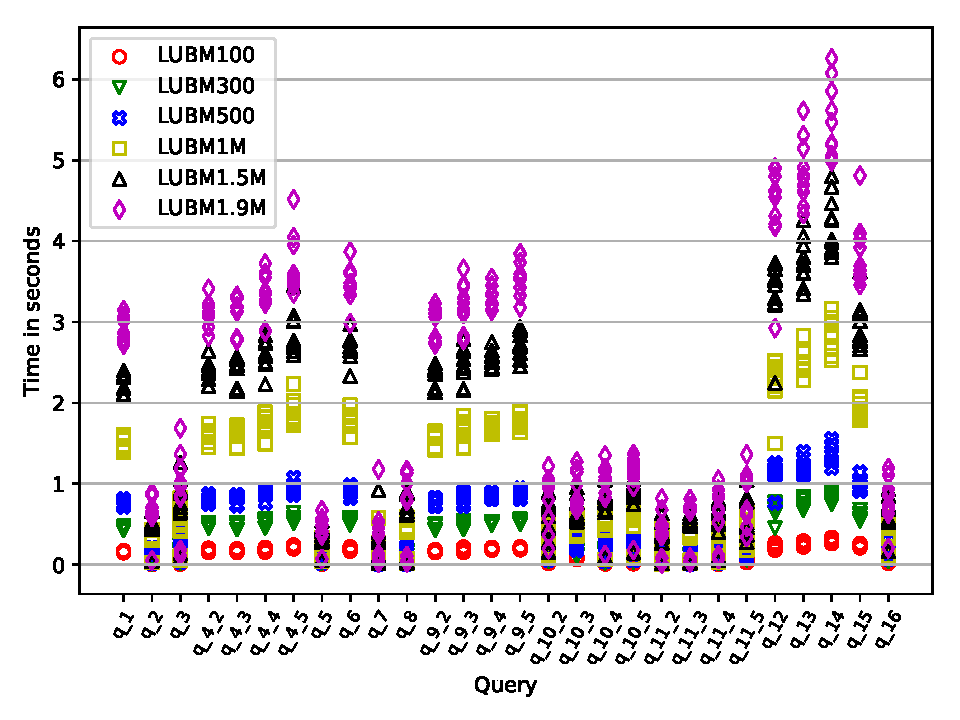
\includegraphics[width=0.48\textwidth]{data/LUBM_all.pdf}
   \caption{Reachability index creation time for LUBM graphs}
   \label{fig:lubm_all_qs}
\end{figure}

Reachability index creation time for each query for for real-world graphs is presented in figure~\ref{fig:other_all_qs}.
We can see that query evaluation time depends on graph inner structure. 
First of all, in some cases handling of small graph requires more time, then handling bigger graph.
For example, $Q_{10}^4$: querying the \textit{geospecies} graph (450k vertices) in some cases requires more time than querying of \textit{mappingbased\_properties} (8.3M vertices) and \textit{taxonomy} (5.7M vertices).
On the other hand, \textit{taxonomy} querying in relatively big number of cases requires significantly more time, than querying of other graphs, while \textit{taxonomy} is not a biggest graph. 
Finally, we can see, that in big number of cases query execution time requires less then 10 seconds, even for big graph, and no queries which require more then 52.17 seconds. 

\begin{figure}
   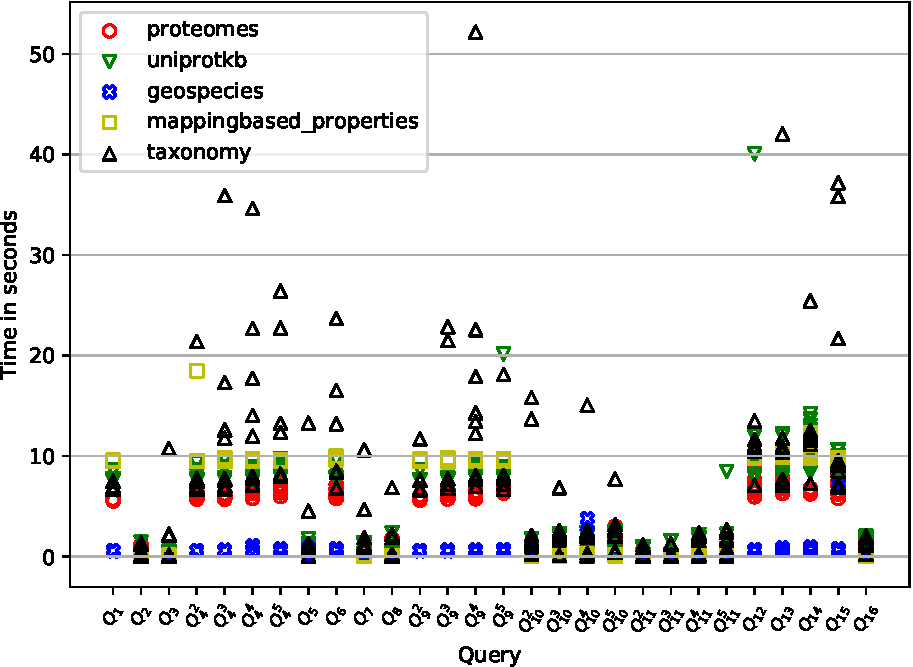
\includegraphics[width=0.48\textwidth]{data/other_all.pdf}
   \caption{Reachability index creation time for real-world RDFs}
   \label{fig:other_all_qs}
\end{figure}

Paths extraction was evaluated on cases with possible long paths.
These cases were selected during reachability index creation by using number of iterations in transitive closure evaluation.
For each selected graph and query we measure paths extraction time for each reachable pair, reachability index creation time is not included because exactly the same index, as calculated at the previous step, is used for paths extraction. 

We evaluate two scenarios.
The first one is a single path extraction.
In this case results are represented as a dependency of extraction time on extracted path length.
We can see linear !!!!

The second scenario is many paths extraction.
Here we limit a number of path to extract by !!! 
In this case results are represented as a dependency of extraction time on number of extracted paths.


\begin{figure}
     \begin{subfigure}[b]{0.24\textwidth}
         \centering
         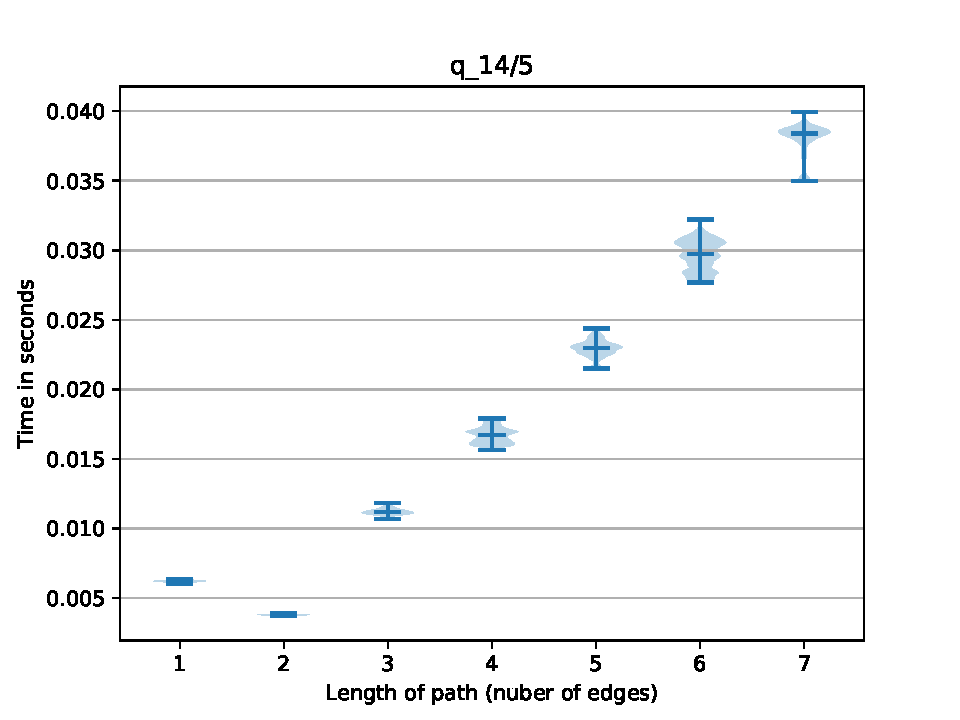
\includegraphics[width=\textwidth]{data/res_graphics/q_14_5.pdf}
         \caption{$y=x$}
         \label{fig:y equals x}
     \end{subfigure}
     ~\begin{subfigure}[b]{0.24\textwidth}
         \centering
         %\includegraphics[width=\textwidth]{data/res_graphics/q9_2_8.pdf}
         \caption{$y=x$}
         \label{fig:y equals x}
     \end{subfigure}\\
     \begin{subfigure}[b]{0.24\textwidth}
         \centering
         %\includegraphics[width=\textwidth]{data/res_graphics/q_14_8.pdf}
         \caption{$y=x$}
         \label{fig:y equals x}
     \end{subfigure}
     ~\begin{subfigure}[b]{0.24\textwidth}
         \centering
         %\includegraphics[width=\textwidth]{data/res_graphics/q4_2_8.pdf}
         \caption{$y=x$}
         \label{fig:y equals x}
     \end{subfigure}
   %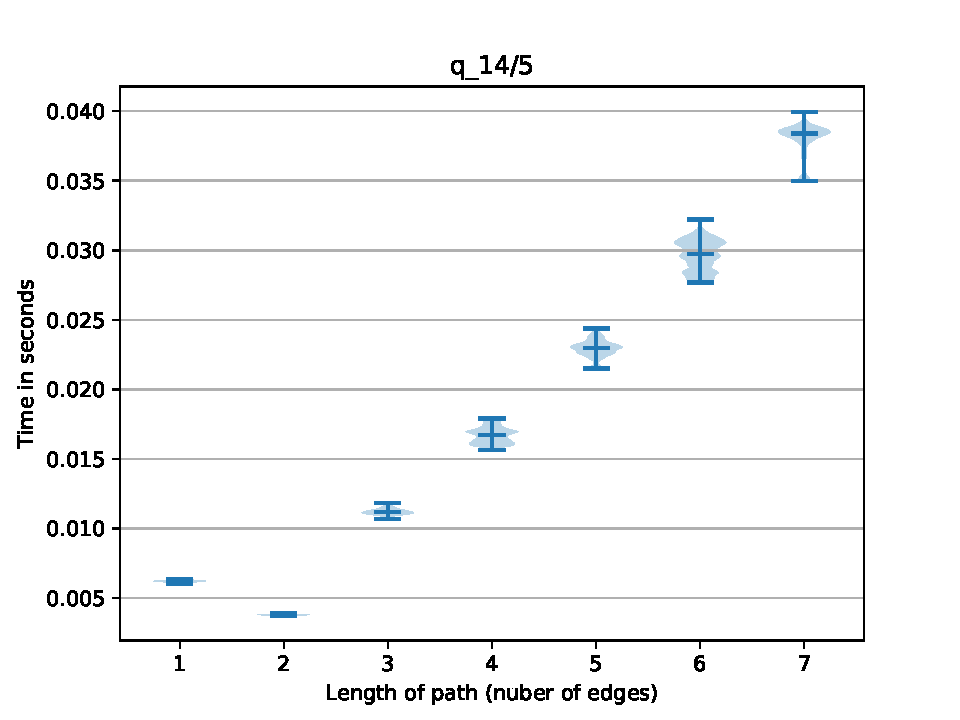
\includegraphics[width=0.48\textwidth]{data/res_graphics/q_14_5.pdf}
   \caption{Single path extraction}
\end{figure}

\subsubsection{Conclusion}

We can conclude that proposed algorithm is applicable for real-world data processing: the algorithm allows one both to solve reachability problem and to extract paths of interest in reasonable time even using na{\"i}ve implementation.  

\subsection{CFPQ Evaluation}

Comparison with matrix-based algorithm.

\subsubsection{Dataset}

Dataset for evaluation. 
It should be CFPQ\_Data\footnote{CFPQ\_Data is a dataset for CFPQ evaluation which contains both synthetic and real-world data and queries \url{https://github.com/JetBrains-Research/CFPQ\_Data}. Access date: 07.07.2020.}

\begin{table}
{
\rowcolors{2}{black!2}{black!10}
\begin{tabular}{|l|c|c|}
\hline
Graph & \#V & \#E \\
\hline
\hline 
eclass\_514en  & 120 926 & 484 646 \\
enzyme  & 358 434 & 144 9711 \\
geospecies  & 596 760 & 2 416 513 \\
go   & 1 188 340 & 4 820 728 \\
go-hierarchy & 1 780 956 & 7 228 358 \\
taxonomy & 2 308 385 & 9 369 511 \\
\hline
Aliases 1 & 6 442 630 & 24 465 430 \\
Aliases 2 & 4 834 262 & 12 366 973 \\
.... & 5 728 398 & 14 922 125 \\
\hline
\end{tabular}
}
\caption{Graphs for CFPQ evaluation}
\label{tbl:graphs_for_cfpq}
\end{table}



Same-generation queries, memory aliases.

\subsubsection{Results}

Results of evaluation.

Index creation.

{\setlength{\tabcolsep}{0.4em}
	\begin{table}
		\caption{RDFs query $G_1$ and $G_2$ (time is measured in seconds and memory is measured in megabytes)}
		\label{tbl:tableRDFQ1_appendix}
		\rowcolors{4}{black!2}{black!10}
		\small
		\begin{tabular}{| l | c | c | c | c |}
			\hline
			
			\multirow{2}{*}{Name}  & \multicolumn{2}{c|}{$G_1$} & \multicolumn{2}{c|}{$G_2$} \\
			\cline{2-5}
			                       & Tensors & RG\_CPU\textsubscript{path} & Tensors & RG\_CPU\textsubscript{path}	 \\
			\hline
			\hline
			eclass\_514en   & 0.254   & 0.195   & 0.227 & ...\\
			enzyme          & 0.035   & 0.029   & 0.036 & ...\\
			geospecies      & 0.091   & ...     & 0.001 & ...\\
			go-hierarchy    & 0.186   & 0.976   & 0.293 & ...\\
			go              & 1.676   & 1.286   & 1.368 & ...\\
			pathways        & 0.015   & 0.021   & 0.009 & ...\\
			taxonomy        & 5.366   & .....   & 3.282 & ...\\
			\hline
		\end{tabular}
	\end{table}
}


Paths extraction.

\subsubsection{Conclusion}

\section{Related Work}

Some different formulation of the similar problems: Language-constrained path querying and language reachability.
Language-constrained path querying, Yannakakis~\cite{Yannakakis}. 
Hellings~\cite{ConjCFPathQuery, Hellings16}, RDF~\cite{CFGonRDF}, etc~\cite{QueryGraphWithData, RegularDBQuery, GraphQueryWithEarley, FLCpathProblem, graphDB}

Special graph query languages. SPARQL, cypher

Languge integration problem: special DSLs for SQL, ORM, Linq.
Transperent integration inpo gp programming language: static correctness, typing.

Parser-combinators is one of classical approach for parsing!!!.

Scala combinators for graph~\cite{ScalaGraphParsing} --- one of attempt to adopt combinators 
technique for graph processing.
Only an idea of combinators using, but language class and restrictions are not discussed.
Problems with cycles in graph. 
Ad-hoc solution. We propose a general solution.
Problems with left-recursive grammars(???Should be checked)

Classical combinators are based on LL(k) and has restrictions: left-recursive grammars.
GLL~\cite{scott2010gll} can handle arbitrary context-free grammars, SPPF~\cite{SPPF}

Parser combinators library bsed on GLL --- 
Meerkat~\footnote{\url{https://github.com/meerkat-parser/Meerkat}}~\cite{Meerkat}. 
Can handle arbitrary context-free grammars
Written in Scala

Structural representation of result: not only reachability, but paths; debuggibg; understanding.
\section{Conclusion and future work}
In this paper, we shown how the context-free path query evaluation w.r.t. the relational and the single-path query semantics can be reduced to the calculation of matrix transitive closure. Also, we provided a formal proof of the correctness of the proposed reduction. In addition, we introduced an algorithm for computing this transitive closure, which allows us to efficiently apply GPGPU computing techniques. Finally, we shown the practical applicability of the proposed algorithm by running different implementations of our algorithm on real-world data.

We can identify several open problems for further research. In this paper we have considered only two semantics of context-free path querying but there are other important semantics, such as all-path query semantics~\cite{hellingsPathQuerying} which requires to present all paths for all triples $(A,m,n)$. Context-free path querying implemented with algorithm~\cite{GLL} can answer the queries in all-path query semantics by constructing a parse forest. It is possible to construct a parse forest for a linear input by matrix multiplication~\cite{okhotin_cyk}. Whether it is possible to generalize this approach for a graph input is an open question.

In our algorithm, we calculate the matrix transitive closure naively, but there are algorithms for the transitive closure calculation, which are asymptotically more efficient. Therefore, the question is whether it is possible to apply these algorithms for the matrix transitive closure calculation to the problem of context-free path querying.

Also, there are Boolean grammars~\cite{okhotinBoolean}, which have more expressive power than context-free grammars. Boolean path querying is an undecidable problem~\cite{hellingsRelational} but our algorithm can be trivially generalized to work on boolean grammars because parsing with boolean grammars can be expressed by matrix multiplication~\cite{okhotin_cyk}. It is not clear what a result of our algorithm applied to Boolean grammars would look like. Our hypothesis is that it would produce the upper approximation of a solution.

From a practical point of view, matrix multiplication in the main loop of the proposed algorithm may be performed on different GPGPU independently. It can help to utilize the power of multi-GPU systems and increase the performance of context-free path querying.

There is an algorithm~\cite{apspGPU} for transitive closure calculation on directed graphs which generalized to handle graph sizes inherently larger then the DRAM memory available on the GPU. Therefore, the question is whether it is possible to apply this approach to the matrix transitive closure calculation in the problem of context-free path querying.
%
{\tiny
getPaths($2,2,S,C_3^6,M_1,M_2^0$) \\
---------getPInner($2,14,C_3^6,M_1,M_2^0$)\\
------------parts$=\{4\}$\\
------------getSubpaths($2,14,4,C_3^6,M_1,M_2^0$)\\
---------------l=$\{2 \xrightarrow{a} 0\}$\\
---------------getPInner($4,14,C_3^6,M_1,M_2^0$)\\
------------------parts=$\{11\}$\\
------------------getSubpaths($4,14,11,C_3^6,M_1,M_2^0$)\\
---------------------getPaths($0,3,S,C_3^6,M_1,M_2^0$)\\
------------------------getPInner($0,15,C_3^6,M_1,M_2^0$))\\
---------------------------parts=$\{5,10\}$\\
---------------------------getSubpaths($0,15,5,C_3^6,M_1,M_2^0$)\\
------------------------------l=$\{0 \xrightarrow{a} 1\}$\\
------------------------------getPInner($5,15,C_3^6,M_1,M_2^0$)\\
---------------------------------parts=$\{10\}$\\
---------------------------------getSubpaths($5,15,10,C_3^6,M_1,M_2^0$)\\
------------------------------------getPaths($1,2,S,C_3^6,M_1,M_2^0$)\\
---------------------------------------getPInner($1,14,C_3^6,M_1,M_2^0$)\\
------------------------------------------parts=$\{6,11\}$\\
------------------------------------------getSubpaths($1,14,6,C_3^6,M_1,M_2^0$)\\
---------------------------------------------l=$\{1 \xrightarrow{a} 2\}$\\
---------------------------------------------getPInner($6,14,C_3^6,M_1,M_2^0$)\\
------------------------------------------------parts=$\{11\}$\\
------------------------------------------------getSubpaths($6,14,11,C_3^6,M_1,M_2^0$)\\
---------------------------------------------------getPaths($2,3,S,C_3^6,M_1,M_2^0$)\\
------------------------------------------------------getPInner($2,15,C_3^6,M_1,M_2^0$)\\
---------------------------------------------------------parts=$\{4,10\}$\\
---------------------------------------------------------getSubpaths($2,15,4,C_3^6,M_1,M_2^0$)\\
------------------------------------------------------------l=$\{2 \xrightarrow{a} 0\}$\\
------------------------------------------------------------getPInner($4,15,C_3^6,M_1,M_2^0$)\\
---------------------------------------------------------------parts=$\{10\}$\\
---------------------------------------------------------------getSubpaths($4,15,10,C_3^6,M_1,M_2^0$)\\
------------------------------------------------------------------getPaths($0,2,S,C_3^6,M_1,M_2^0$)\\
---------------------------------------------------------------------getPInner($0,14,C_3^6,M_1,M_2^0$)\\
------------------------------------------------------------------------parts=$\{5,11\}$\\
------------------------------------------------------------------------getSubpaths($0,14,5,C_3^6,M_1,M_2^0$)\\
---------------------------------------------------------------------------l=$\{0 \xrightarrow{a} 1\}$\\
---------------------------------------------------------------------------getPInner($5,14,C_3^6,M_1,M_2^0$)\\
------------------------------------------------------------------------------parts=$\{11\}$\\
------------------------------------------------------------------------------getSubpaths($5,14,11,C_3^6,M_1,M_2^0$)\\
---------------------------------------------------------------------------------getPaths($1,3,S,C_3^6,M_1,M_2^0$)\\
------------------------------------------------------------------------------------getPInner($1,15,C_3^6,M_1,M_2^0$)\\
---------------------------------------------------------------------------------------parts=$\{6\}$\\
---------------------------------------------------------------------------------------getSubpaths($1,15,6,C_3^6,M_1,M_2^0$)\\
------------------------------------------------------------------------------------------l = $\{1 \xrightarrow{a} 2\}$\\
------------------------------------------------------------------------------------------r = $\{2 \xrightarrow{b} 3\}$\\
------------------------------------------------------------------------------------------$l\cdot r = \{1 \xrightarrow{a} 2 \xrightarrow{b} 3\}$\\ 
---------------------------------------------------------------------------------------$\{1 \xrightarrow{a} 2 \xrightarrow{b} 3\}$\\
------------------------------------------------------------------------------------$\{1 \xrightarrow{a} 2 \xrightarrow{b} 3\}$\\
---------------------------------------------------------------------------------l=$\{1 \xrightarrow{a} 2 \xrightarrow{b} 3\}$\\
---------------------------------------------------------------------------------r=$\{3 \xrightarrow{b} 2\}$\\
---------------------------------------------------------------------------------$l \cdot r = \{1 \xrightarrow{a} 2 \xrightarrow{b} 3 \xrightarrow{b} 2\}$\\
------------------------------------------------------------------------------$\{1 \xrightarrow{a} 2 \xrightarrow{b} 3 \xrightarrow{b} 2\}$\\
---------------------------------------------------------------------------r = $\{1 \xrightarrow{a} 2 \xrightarrow{b} 3 \xrightarrow{b} 2\}$\\
---------------------------------------------------------------------------$l \cdot r = \{0 \xrightarrow{a} 1 \xrightarrow{a} 2 \xrightarrow{b} 3 \xrightarrow{b} 2\}$\\
------------------------------------------------------------------------getSubpaths($0,14,11,C_3^6,M_1,M_2^0$)\\
---------------------------------------------------------------------------getPInner($0,11,C_3^6,M_1,M_2^0$)\\
------------------------------------------------------------------------------parts=$\{5\}$\\
------------------------------------------------------------------------------getSubpaths($0,11,5,C_3^6,M_1,M_2^0$)\\
---------------------------------------------------------------------------------l=$\{0 \xrightarrow{a} 1\}$\\
---------------------------------------------------------------------------------getPaths($1,3,S,C_3^6,M_1,M_2^0$) (*recursive call!!! Infinite set of paths*)\\
---------------------------------------------------------------------------------r = $r_\infty^{1\leadsto 3}$\\
---------------------------------------------------------------------------------$l \cdot r = \{0 \xrightarrow{a} 1\} \cdot r_\infty^{1\leadsto 3}$\\
------------------------------------------------------------------------------$\{0 \xrightarrow{a} 1\} \cdot r_\infty^{1\leadsto 3}$\\
---------------------------------------------------------------------------l =  $\{0 \xrightarrow{a} 1\} \cdot r_\infty^{1\leadsto 3}$\\
---------------------------------------------------------------------------r = $\{3 \xrightarrow{b} 2\}$\\
---------------------------------------------------------------------------$l \cdot r = \{0 \xrightarrow{a} 1\} \cdot r_\infty^{1\leadsto 3} \cdot \{3 \xrightarrow{b} 2\}$\\
------------------------------------------------------------------------$\{0 \xrightarrow{a} 1 \xrightarrow{a} 2 \xrightarrow{b} 3 \xrightarrow{b} 2\} \cup (\{0 \xrightarrow{a} 1\} \cdot r_\infty^{1\leadsto 3} \cdot \{3 \xrightarrow{b} 2\})$\\
---------------------------------------------------------------------$\{0 \xrightarrow{a} 1 \xrightarrow{a} 2 \xrightarrow{b} 3 \xrightarrow{b} 2\} \cup (\{0 \xrightarrow{a} 1\} \cdot r_\infty^{1\leadsto 3} \cdot \{3 \xrightarrow{b} 2\})$\\
------------------------------------------------------------------l=$\{0 \xrightarrow{a} 1 \xrightarrow{a} 2 \xrightarrow{b} 3 \xrightarrow{b} 2\} \cup (\{0 \xrightarrow{a} 1\} \cdot r_\infty^{1\leadsto 3} \cdot \{3 \xrightarrow{b} 2\})$\\
------------------------------------------------------------------r=$\{2 \xrightarrow{b} 3\}$\\
------------------------------------------------------------------$l \cdot r = \{0 \xrightarrow{a} 1 \xrightarrow{a} 2 \xrightarrow{b} 3 \xrightarrow{b} 2 \xrightarrow{b} 3\} \cup (\{0 \xrightarrow{a} 1\} \cdot r_\infty^{1\leadsto 3} \cdot \{3 \xrightarrow{b} 2 \xrightarrow{b} 3\})$\\
---------------------------------------------------------------$\{0 \xrightarrow{a} 1 \xrightarrow{a} 2 \xrightarrow{b} 3 \xrightarrow{b} 2 \xrightarrow{b} 3\} \cup (\{0 \xrightarrow{a} 1\} \cdot r_\infty^{1\leadsto 3} \cdot \{3 \xrightarrow{b} 2 \xrightarrow{b} 3\})$\\
------------------------------------------------------------r=$\{0 \xrightarrow{a} 1 \xrightarrow{a} 2 \xrightarrow{b} 3 \xrightarrow{b} 2 \xrightarrow{b} 3\} \cup (\{0 \xrightarrow{a} 1\} \cdot r_\infty^{1\leadsto 3} \cdot \{3 \xrightarrow{b} 2 \xrightarrow{b} 3\})$\\
------------------------------------------------------------$l \cdot r = \{\{2 \xrightarrow{a} 0 \xrightarrow{a} 1 \xrightarrow{a} 2 \xrightarrow{b} 3 \xrightarrow{b} 2 \xrightarrow{b} 3\} \cup (\{2 \xrightarrow{a} 0 \xrightarrow{a} 1\} \cdot r_\infty^{1\leadsto 3} \cdot \{3 \xrightarrow{b} 2 \xrightarrow{b} 3\})$\\

---------------------------------------------------------getSubpaths($2,15,10,C_3^6,M_1,M_2^0$)\\
------------------------------------------------------------getPInner($2,10,C_3^6,M_1,M_2^0$)\\
---------------------------------------------------------------parts=$\{4\}$\\
---------------------------------------------------------------getSubpaths($2,10,4,C_3^6,M_1,M_2^0$)\\
------------------------------------------------------------------l=$\{2 \xrightarrow{a} 0\}$\\
------------------------------------------------------------------getPaths($0,2,S,C_3^6,M_1,M_2^0$)(*recursive call!!! Infinite set of paths*)\\
------------------------------------------------------------------$r = r_\infty^{0\leadsto 2}$\\
------------------------------------------------------------------$l \cdot r = \{2 \xrightarrow{a} 0\} \cdot r_\infty^{0\leadsto 2}$\\
---------------------------------------------------------------$\{2 \xrightarrow{a} 0\} \cdot r_\infty^{0\leadsto 2}$\\
------------------------------------------------------------l=$\{2 \xrightarrow{a} 0\} \cdot r_\infty^{0\leadsto 2}$\\
------------------------------------------------------------r=$\{2 \xrightarrow{b} 3\}$\\
------------------------------------------------------------$l \cdot r =\{2 \xrightarrow{a} 0\} \cdot r_\infty^{0\leadsto 2} \cdot \{2 \xrightarrow{b} 3\} $\\
------------------------------------------------------$\{2 \xrightarrow{a} 0 \xrightarrow{a} 1 \xrightarrow{a} 2 \xrightarrow{b} 3 \xrightarrow{b} 2 \xrightarrow{b} 3\} \cup (\{2 \xrightarrow{a} 0 \xrightarrow{a} 1\} \cdot r_\infty^{1\leadsto 3} \cdot \{3 \xrightarrow{b} 2 \xrightarrow{b} 3\}) \cup (\{2 \xrightarrow{a} 0\} \cdot r_\infty^{0\leadsto 2} \cdot \{2 \xrightarrow{b} 3\})$ (*last is the same as middle so omit it in our example*)\\
---------------------------------------------------l=$\{2 \xrightarrow{a} 0 \xrightarrow{a} 1 \xrightarrow{a} 2 \xrightarrow{b} 3 \xrightarrow{b} 2 \xrightarrow{b} 3\} \cup (\{2 \xrightarrow{a} 0 \xrightarrow{a} 1\} \cdot r_\infty^{1\leadsto 3} \cdot \{3 \xrightarrow{b} 2 \xrightarrow{b} 3\}))$\\
---------------------------------------------------r=$\{3 \xrightarrow{b} 2\}$\\
---------------------------------------------------$l \cdot r =\{2 \xrightarrow{a} 0 \xrightarrow{a} 1 \xrightarrow{a} 2 \xrightarrow{b} 3 \xrightarrow{b} 2 \xrightarrow{b} 3 \xrightarrow{b} 2\} \cup (\{2 \xrightarrow{a} 0 \xrightarrow{a} 1\} \cdot r_\infty^{1\leadsto 3} \cdot \{3 \xrightarrow{b} 2 \xrightarrow{b} 3 \xrightarrow{b} 2\}))$\\
------------------------------------------------$\{2 \xrightarrow{a} 0 \xrightarrow{a} 1 \xrightarrow{a} 2 \xrightarrow{b} 3 \xrightarrow{b} 2 \xrightarrow{b} 3 \xrightarrow{b} 2\} \cup (\{2 \xrightarrow{a} 0 \xrightarrow{a} 1\} \cdot r_\infty^{1\leadsto 3} \cdot \{3 \xrightarrow{b} 2 \xrightarrow{b} 3 \xrightarrow{b} 2\}))$\\
---------------------------------------------r=$\{2 \xrightarrow{a} 0 \xrightarrow{a} 1 \xrightarrow{a} 2 \xrightarrow{b} 3 \xrightarrow{b} 2 \xrightarrow{b} 3 \xrightarrow{b} 2\} \cup (\{2 \xrightarrow{a} 0 \xrightarrow{a} 1\} \cdot r_\infty^{1\leadsto 3} \cdot \{3 \xrightarrow{b} 2 \xrightarrow{b} 3 \xrightarrow{b} 2\}))$\\
---------------------------------------------$l\cdot r = \{1 \xrightarrow{a} 2 \xrightarrow{a} 0 \xrightarrow{a} 1 \xrightarrow{a} 2 \xrightarrow{b} 3 \xrightarrow{b} 2 \xrightarrow{b} 3 \xrightarrow{b} 2\} \cup (1 \xrightarrow{a} 2 \xrightarrow{a} 0 \xrightarrow{a} 1\} \cdot r_\infty^{1\leadsto 3} \cdot \{3 \xrightarrow{b} 2 \xrightarrow{b} 3 \xrightarrow{b} 2\}))$\\
------------------------------------------getSubpaths($1,14,11,C_3^6,M_1,M_2^0$) (*Leads to recursion. Omited*)\\
------------------------------------------$\{1 \xrightarrow{a} 2 \xrightarrow{a} 0 \xrightarrow{a} 1 \xrightarrow{a} 2 \xrightarrow{b} 3 \xrightarrow{b} 2 \xrightarrow{b} 3 \xrightarrow{b} 2\} \cup (1 \xrightarrow{a} 2 \xrightarrow{a} 0 \xrightarrow{a} 1\} \cdot r_\infty^{1\leadsto 3} \cdot \{3 \xrightarrow{b} 2 \xrightarrow{b} 3 \xrightarrow{b} 2\}))$\\
---------------------------------------$\{1 \xrightarrow{a} 2 \xrightarrow{a} 0 \xrightarrow{a} 1 \xrightarrow{a} 2 \xrightarrow{b} 3 \xrightarrow{b} 2 \xrightarrow{b} 3 \xrightarrow{b} 2\} \cup (1 \xrightarrow{a} 2 \xrightarrow{a} 0 \xrightarrow{a} 1\} \cdot r_\infty^{1\leadsto 3} \cdot \{3 \xrightarrow{b} 2 \xrightarrow{b} 3 \xrightarrow{b} 2\}))$\\
------------------------------------l=$\{1 \xrightarrow{a} 2 \xrightarrow{a} 0 \xrightarrow{a} 1 \xrightarrow{a} 2 \xrightarrow{b} 3 \xrightarrow{b} 2 \xrightarrow{b} 3 \xrightarrow{b} 2\} \cup (1 \xrightarrow{a} 2 \xrightarrow{a} 0 \xrightarrow{a} 1\} \cdot r_\infty^{1\leadsto 3} \cdot \{3 \xrightarrow{b} 2 \xrightarrow{b} 3 \xrightarrow{b} 2\}))$\\
------------------------------------r=$\{2 \xrightarrow{b} 3\}$\\
------------------------------------$l\cdot r = \{1 \xrightarrow{a} 2 \xrightarrow{a} 0 \xrightarrow{a} 1 \xrightarrow{a} 2 \xrightarrow{b} 3 \xrightarrow{b} 2 \xrightarrow{b} 3 \xrightarrow{b} 2 \xrightarrow{b} 3\} \cup (1 \xrightarrow{a} 2 \xrightarrow{a} 0 \xrightarrow{a} 1\} \cdot r_\infty^{1\leadsto 3} \cdot \{3 \xrightarrow{b} 2 \xrightarrow{b} 3 \xrightarrow{b} 2 \xrightarrow{b} 3\}))$\\
---------------------------------$\{1 \xrightarrow{a} 2 \xrightarrow{a} 0 \xrightarrow{a} 1 \xrightarrow{a} 2 \xrightarrow{b} 3 \xrightarrow{b} 2 \xrightarrow{b} 3 \xrightarrow{b} 2 \xrightarrow{b} 3\} \cup (1 \xrightarrow{a} 2 \xrightarrow{a} 0 \xrightarrow{a} 1\} \cdot r_\infty^{1\leadsto 3} \cdot \{3 \xrightarrow{b} 2 \xrightarrow{b} 3 \xrightarrow{b} 2 \xrightarrow{b} 3\}))$\\
------------------------------r=$\{1 \xrightarrow{a} 2 \xrightarrow{a} 0 \xrightarrow{a} 1 \xrightarrow{a} 2 \xrightarrow{b} 3 \xrightarrow{b} 2 \xrightarrow{b} 3 \xrightarrow{b} 2 \xrightarrow{b} 3\} \cup (1 \xrightarrow{a} 2 \xrightarrow{a} 0 \xrightarrow{a} 1\} \cdot r_\infty^{1\leadsto 3} \cdot \{3 \xrightarrow{b} 2 \xrightarrow{b} 3 \xrightarrow{b} 2 \xrightarrow{b} 3\}))$\\
------------------------------$l \cdot r = \{0 \xrightarrow{a} 1 \xrightarrow{a} 2 \xrightarrow{a} 0 \xrightarrow{a} 1 \xrightarrow{a} 2 \xrightarrow{b} 3 \xrightarrow{b} 2 \xrightarrow{b} 3 \xrightarrow{b} 2 \xrightarrow{b} 3\} \cup (0 \xrightarrow{a} 1 \xrightarrow{a} 2 \xrightarrow{a} 0 \xrightarrow{a} 1\} \cdot r_\infty^{1\leadsto 3} \cdot \{3 \xrightarrow{b} 2 \xrightarrow{b} 3 \xrightarrow{b} 2 \xrightarrow{b} 3\}))$\\
---------------------------getSubpaths($0,15,10,C_3^6,M_1,M_2^0$) (*Leads to recursion. Omited*)\\
---------------------------$\{0 \xrightarrow{a} 1 \xrightarrow{a} 2 \xrightarrow{a} 0 \xrightarrow{a} 1 \xrightarrow{a} 2 \xrightarrow{b} 3 \xrightarrow{b} 2 \xrightarrow{b} 3 \xrightarrow{b} 2 \xrightarrow{b} 3\} \cup (0 \xrightarrow{a} 1 \xrightarrow{a} 2 \xrightarrow{a} 0 \xrightarrow{a} 1\} \cdot r_\infty^{1\leadsto 3} \cdot \{3 \xrightarrow{b} 2 \xrightarrow{b} 3 \xrightarrow{b} 2 \xrightarrow{b} 3\}))$\\
------------------------$\{0 \xrightarrow{a} 1 \xrightarrow{a} 2 \xrightarrow{a} 0 \xrightarrow{a} 1 \xrightarrow{a} 2 \xrightarrow{b} 3 \xrightarrow{b} 2 \xrightarrow{b} 3 \xrightarrow{b} 2 \xrightarrow{b} 3\} \cup (0 \xrightarrow{a} 1 \xrightarrow{a} 2 \xrightarrow{a} 0 \xrightarrow{a} 1\} \cdot r_\infty^{1\leadsto 3} \cdot \{3 \xrightarrow{b} 2 \xrightarrow{b} 3 \xrightarrow{b} 2 \xrightarrow{b} 3\}))$\\
---------------------l=$\{0 \xrightarrow{a} 1 \xrightarrow{a} 2 \xrightarrow{a} 0 \xrightarrow{a} 1 \xrightarrow{a} 2 \xrightarrow{b} 3 \xrightarrow{b} 2 \xrightarrow{b} 3 \xrightarrow{b} 2 \xrightarrow{b} 3\} \cup (0 \xrightarrow{a} 1 \xrightarrow{a} 2 \xrightarrow{a} 0 \xrightarrow{a} 1\} \cdot r_\infty^{1\leadsto 3} \cdot \{3 \xrightarrow{b} 2 \xrightarrow{b} 3 \xrightarrow{b} 2 \xrightarrow{b} 3\}))$\\
---------------------r=$\{3 \xrightarrow{b} 2\}$\\
---------------------$l\cdot r = \{0 \xrightarrow{a} 1 \xrightarrow{a} 2 \xrightarrow{a} 0 \xrightarrow{a} 1 \xrightarrow{a} 2 \xrightarrow{b} 3 \xrightarrow{b} 2 \xrightarrow{b} 3 \xrightarrow{b} 2 \xrightarrow{b} 3 \xrightarrow{b} 2\} \cup (0 \xrightarrow{a} 1 \xrightarrow{a} 2 \xrightarrow{a} 0 \xrightarrow{a} 1\} \cdot r_\infty^{1\leadsto 3} \cdot \{3 \xrightarrow{b} 2 \xrightarrow{b} 3 \xrightarrow{b} 2 \xrightarrow{b} 3 \xrightarrow{b} 2\}))$\\
------------------$\{0 \xrightarrow{a} 1 \xrightarrow{a} 2 \xrightarrow{a} 0 \xrightarrow{a} 1 \xrightarrow{a} 2 \xrightarrow{b} 3 \xrightarrow{b} 2 \xrightarrow{b} 3 \xrightarrow{b} 2 \xrightarrow{b} 3 \xrightarrow{b} 2\} \cup (0 \xrightarrow{a} 1 \xrightarrow{a} 2 \xrightarrow{a} 0 \xrightarrow{a} 1\} \cdot r_\infty^{1\leadsto 3} \cdot \{3 \xrightarrow{b} 2 \xrightarrow{b} 3 \xrightarrow{b} 2 \xrightarrow{b} 3 \xrightarrow{b} 2\}))$\\
---------------r=$\{0 \xrightarrow{a} 1 \xrightarrow{a} 2 \xrightarrow{a} 0 \xrightarrow{a} 1 \xrightarrow{a} 2 \xrightarrow{b} 3 \xrightarrow{b} 2 \xrightarrow{b} 3 \xrightarrow{b} 2 \xrightarrow{b} 3 \xrightarrow{b} 2\} \cup (0 \xrightarrow{a} 1 \xrightarrow{a} 2 \xrightarrow{a} 0 \xrightarrow{a} 1\} \cdot r_\infty^{1\leadsto 3} \cdot \{3 \xrightarrow{b} 2 \xrightarrow{b} 3 \xrightarrow{b} 2 \xrightarrow{b} 3 \xrightarrow{b} 2\}))$\\
---------------$l \cdot r = \{2 \xrightarrow{a} 0 \xrightarrow{a} 1 \xrightarrow{a} 2 \xrightarrow{a} 0 \xrightarrow{a} 1 \xrightarrow{a} 2 \xrightarrow{b} 3 \xrightarrow{b} 2 \xrightarrow{b} 3 \xrightarrow{b} 2 \xrightarrow{b} 3 \xrightarrow{b} 2\} \cup (2 \xrightarrow{a}  0 \xrightarrow{a} 1 \xrightarrow{a} 2 \xrightarrow{a} 0 \xrightarrow{a} 1\} \cdot r_\infty^{1\leadsto 3} \cdot \{3 \xrightarrow{b} 2 \xrightarrow{b} 3 \xrightarrow{b} 2 \xrightarrow{b} 3 \xrightarrow{b} 2\}))$\\
------------$\{2 \xrightarrow{a} 0 \xrightarrow{a} 1 \xrightarrow{a} 2 \xrightarrow{a} 0 \xrightarrow{a} 1 \xrightarrow{a} 2 \xrightarrow{b} 3 \xrightarrow{b} 2 \xrightarrow{b} 3 \xrightarrow{b} 2 \xrightarrow{b} 3 \xrightarrow{b} 2\} \cup (2 \xrightarrow{a}  0 \xrightarrow{a} 1 \xrightarrow{a} 2 \xrightarrow{a} 0 \xrightarrow{a} 1\} \cdot r_\infty^{1\leadsto 3} \cdot \{3 \xrightarrow{b} 2 \xrightarrow{b} 3 \xrightarrow{b} 2 \xrightarrow{b} 3 \xrightarrow{b} 2\}))$\\
---------$\{2 \xrightarrow{a} 0 \xrightarrow{a} 1 \xrightarrow{a} 2 \xrightarrow{a} 0 \xrightarrow{a} 1 \xrightarrow{a} 2 \xrightarrow{b} 3 \xrightarrow{b} 2 \xrightarrow{b} 3 \xrightarrow{b} 2 \xrightarrow{b} 3 \xrightarrow{b} 2\} \cup (2 \xrightarrow{a}  0 \xrightarrow{a} 1 \xrightarrow{a} 2 \xrightarrow{a} 0 \xrightarrow{a} 1\} \cdot r_\infty^{1\leadsto 3} \cdot \{3 \xrightarrow{b} 2 \xrightarrow{b} 3 \xrightarrow{b} 2 \xrightarrow{b} 3 \xrightarrow{b} 2\}))$\\

}


%
% The next two lines define the bibliography style to be used, and the bibliography file.
\bibliographystyle{ACM-Reference-Format}
\bibliography{tensor_product_CFPQ}

%
% If your work has an appendix, this is the place to put it.
%\vspace{10cm}


\end{document}
